% This must be in the first 5 lines to tell arXiv to use pdfLaTeX, which is strongly recommended.
\pdfoutput=1
% In particular, the hyperref package requires pdfLaTeX in order to break URLs across lines.

\documentclass[11pt]{article}

% Remove the "review" option to generate the final version.
\usepackage{EMNLP2023}

% Standard package includes
\usepackage{times}
\usepackage{latexsym}
\usepackage{graphicx}%
% \usepackage{tabularx}
% \usepackage{tabulary}
\usepackage{array}
\usepackage{multirow}%
\usepackage{amsmath,amssymb,amsfonts}%
\usepackage{amsthm}%
\usepackage{mathrsfs}%
\usepackage[title]{appendix}%
\usepackage{xcolor}%
\usepackage{textcomp}%
\usepackage{manyfoot}%
\usepackage{booktabs}%
\usepackage{hhline}
\usepackage{algorithm}%
\usepackage{algorithmicx}%
\usepackage{algpseudocode}%
\usepackage{listings}%
\usepackage[caption=false,font=normalsize,labelfont=sf,textfont=sf]{subfig}
\usepackage{stfloats}
\usepackage{url}
\usepackage{verbatim}
 \usepackage{booktabs}
 \usepackage{cite}
\usepackage{hyperref}
\hypersetup{
    colorlinks=true,
    linkcolor=black,
    filecolor=black,      
    urlcolor=black,
    citecolor=blue,
}
\usepackage{cleveref}
\usepackage{balance}
\usepackage{subcaption}
\newcounter{myverb}
\BeforeBeginEnvironment{verbatim}{%
\refstepcounter{myverb}%
\noindent\textbf{Prompt \themyverb}%
}

\setcounter{secnumdepth}{3}% Number up to \subsubsection
\usepackage[T1]{fontenc}
\usepackage[utf8]{inputenc}
\usepackage{microtype}
\usepackage{inconsolata}
\usepackage{newunicodechar}
\usepackage{placeins}
\newunicodechar{−}{-} % replace the actual U+2212 with ASCII hyphen





\title{BitMar: Low-Bit Multimodal Fusion with Episodic Memory for Edge Devices}

% Author information can be set in various styles:
% For several authors from the same institution:
% \author{Author 1 \and ... \and Author n \\
%         Address line \\ ... \\ Address line}
% if the names do not fit well on one line use
%         Author 1 \\ {\bf Author 2} \\ ... \\ {\bf Author n} \\
% For authors from different institutions:
% \author{Author 1 \\ Address line \\  ... \\ Address line
%         \And  ... \And
%         Author n \\ Address line \\ ... \\ Address line}
% To start a separate ``row'' of authors use \AND, as in
% \author{Author 1 \\ Address line \\  ... \\ Address line
%         \AND
%         Author 2 \\ Address line \\ ... \\ Address line \And
%         Author 3 \\ Address line \\ ... \\ Address line}

\author{
  Euhid Aman \\
  NTUST Taiwan \\
  \small \texttt{M11315803@mail.ntust.edu.tw}
  \And
  Esteban Carlin \\
  NTUST Taiwan \\
  \small \texttt{M11302809@mail.ntust.edu.tw}
  \And
  Hsing-Kuo Pao \\
  NTUST Taiwan \\
  \small \texttt{pao@mail.ntust.edu.tw}
  \AND
  Giovanni Beltrame \\
  Polytechnique Montréal \\
  \small \texttt{giovanni.beltrame@polymtl.ca}
  \And
  Ghaluh Indah Permata Sari \\
  NTUST Taiwan \\
  \small \texttt{d11115804@mail.ntust.edu.tw}
  \And
  Yie-Tarng Chen \\
  NTUST Taiwan \\
  \small \texttt{ytchen@mail.ntust.edu.tw}
}



\begin{document}
\maketitle

\begin{abstract}
Cross-attention transformers and other multimodal vision-language models excel at grounding and generation; however, their extensive, full-precision backbones make it challenging to deploy them on edge devices. Memory-augmented architectures enhance the utilization of past context; however, most works rarely pair them with aggressive edge-oriented quantization. We introduce BitMar, a quantized multimodal transformer that proposes an external human-like episodic memory for effective image-text generation on hardware with limited resources. BitMar utilizes 1.58-bit encoders, one for text (BitNet-style) and one for vision (DiNOv2-based), to create compact embeddings that are combined and used to query a fixed-size key-value episodic memory. During vector retrieval, the BitNet decoder applies per‑layer conditioning, which increases the contextual relevance of generated content. The decoder also employs attention sinks with a sliding‑window mechanism to process long or streaming inputs under tight memory budgets. The combination of per-layer conditioning and sliding-window attention achieves a strong quality–speed trade–off, delivering competitive captioning and multimodal understanding at low latency with a small model footprint. These characteristics make BitMar well-suited for edge deployment.




%TOO LONG
% Cross-attention transformers and other multimodal vision-language models excel at grounding and generation. However, they typically require full-precision, large-capacity backbones, which makes them challenging to deploy on devices with limited resources. At the same time, memory-augmented architectures can facilitate the utilization of context over time. However, most systems do not combine them with aggressive quantization that is well-suited for edge settings. This paper presents BitMar, a novel quantized multimodal transformer architecture that integrates human-like episodic memory for efficient cross-modal understanding and generation on edge devices. The model comprises parallel quantized encoders for language and vision: a BitNet-style text encoder and a DiNOv2-based vision encoder, both operating with 1.58-bit weight quantization to minimize computational and memory overhead. Each encoder produces a 768-dimensional latent representation, which is fused via a lightweight cross-modal interaction module to form a unified multimodal embedding. This embedding serves as a query to a human-like episodic memory module implemented as a fixed-size key–value matrix, enabling retrieval of contextually relevant representations from prior data episodes. Retrieved memory vectors are projected into per-layer conditioning signals that modulate a BitNet decoder, allowing generation to be informed by both the current multimodal input and accumulated episodic knowledge. Furthermore, to support unbounded context lengths without growing resource usage, attention sinks are injected while maintaining a sliding window over the most recent tokens. This design achieves a balance between representational capacity and deployment efficiency, supporting competitive multimodal understanding and text generation performance while maintaining low latency and a compact model footprint suitable for edge deployment scenarios.
\end{abstract}

% \newenvironment{keyword}{\begin{center}\bfseries Keywords:Sentence Simplification \sep Generative Model \sep Large Language Model \sep Dual Latent.}{\end{center}}
\noindent\textbf{Keywords:} TinyVLM, Episodic memory, EdgeAI, Quantization.
\section{Introduction}
\label{sec:intro}
Visual Language Models (VLMs) have made rapid progress in recent years, excelling at tasks such as image captioning~\citep{chen-microsoftcoco-2015}, visual question answering~\citep{anderson-attentionimagecap-2018, lijunan-blip-2022}. %and grounded dialogue generation~\citep{alayrac-flamingo-2022}. 
Large-scale architectures such as BLIP-2~\citep{lijunnan-blip2-2023}, Flamingo~\citep{alayrac-flamingo-2022}, and Kosmos-2~\citep{peng-kosmos2-2023} demonstrate that cross-attention transformers can synchronize modalities for grounded language generation. However, their full-precision, extensive backbones incur significant computational and memory expenses, which restricts their implementation on devices with resource limitations.

A growing body of work targets efficient multimodal processing, such as low-bit quantization~\citep{dettmers-8bitquantization-2021, frantar-gptq-2022} and compact language models~\citep{wang-bitnet-2023}, to reduce memory/latency. Quantized ViTs~\citep{jacob-quantization-2018, stock-revisiting-2019}, and self-supervised vision encoders, such as DiNOv2~\citep{oquab-dinov2-2024}, lower the cost of vision. Multimodal fusion ranges from early concatenation~\citep{lu-vilbert-2019} to learned query transformers~\citep{lijunnan-blip2-2023} to bridge frozen vision and language models. Memory-augmented transformers~\citep{graves-dynamicexternalmemory-2016, borgeaud-trillionstokens-2022} retrieve past context to improve coherence. 
Yet no existing tiny language model effectively unifies low-bit multimodal encoding with an episodic memory system for edge deployment.


% A growing body of work explores efficient multimodal processing. On the language side, low-bit quantization methods~\citep{dettmers-8bitquntization-2022, frantar-gptq-2022} and compact architectures such as~\citep{wang-bitnet-2023} significantly reduce memory footprint and inference latency. For vision encoders, quantized ViT variants\citep{jacob-quantization-2018, stock-revisiting-2019} and self-supervised models like DiNOv2~\citep{oquab-dinov2-2024} enable strong visual representations at a lower cost. In multimodal fusion, approaches range from early concatenation~\citep{lu-vilbert-2019} to learned query transformers (BLIP-2) that bridge frozen vision and language models. Memory-augmented transformers\citep{graves-dynamicexternalmemory-2016, borgeaud-trillionstokens-2022} extend these designs by allowing models to store and retrieve past context, improving coherence in sequential or episodic tasks. This follows the idea of human episodic memory, where the hippocampus serves as a short-term memory store enabling rapid and context-aware interactions. Yet, currently, no tiny LLMs combine low-bit multimodal encoding with episodic memory retrieval in a unified, edge-deployable architecture.

% In this work, we propose a compact multimodal generation pipeline built around four stages: two low-bit encoders → cross-modal fusion → episodic memory → BitNet decoder with per-layer memory conditioning. Both the text and vision encoders operate at 1.58-bit quantization, producing 768-dimensional latent vectors that are fused via a lightweight cross-modal interaction layer. The fused multimodal embedding queries a fixed-size episodic memory of 512 slots, retrieving contextually relevant vectors that are projected into layer-specific conditioning signals for the BitNet decoder. This design ensures that all modules operate within a consistent 768-dimensional space, simplifying integration while minimizing projection overhead. 





% We suggest a small four-stage pipeline: (1) 1.58-bit text/vision encoders → (2) lightweight cross-modal fusion → (3) an episodic memory with 512 slots → (4) a BitNet decoder that works with each layer. Both encoders produce 128-dimensional latents, and we compress DiNOv2's original 768-D vision features to 128-D before fusion. 
% The fused embedding queries a $K=512$, $C=128$ episodic memory, and the retrieved vectors condition each decoder layer, keeping all modules in a consistent 768-dimensional space to make integration easier and reduce projection overhead. Our contributions are threefold:

% \begin{itemize}
%     \item We introduce a low-bit multimodal encoding framework that combines a quantized BitNet text encoder and a quantized ViT-based vision encoder for efficient feature extraction.
%     \item We develop a memory-augmented decoding mechanism that injects retrieved episodic context into each transformer layer via per-layer conditioning, improving contextual relevance in caption generation.
%     \item We demonstrate competitive captioning and multimodal understanding under extreme compression, with low latency and a small footprint, making it suitable for edge deployment.%that our architecture can caption images as well as the best ones while using limited memory and having low latency, making it robust for use in edge environments.
% \end{itemize}

% We organize the rest of the paper as follows: some studies on human-centric learning for language models and neural networks in~\autoref{sec:relworks}, ~\autoref{sec:method} describes the proposed model components, ~\autoref{sec:exp} explains the experimental setup, ~\autoref{sec:result} presents and discusses the results, and ~\autoref{sec:conclusion} concludes the paper.










To fill this gap, we propose a compact four-stage pipeline optimized for efficient on-device execution: 
(1) \textbf{1.58-bit text and vision encoders} generate lightweight, quantized embeddings; 
(2) \textbf{a cross-modal fusion module} aligns the modalities within a shared latent space; 
(3) \textbf{an episodic memory} with 512 key--value slots retrieves relevant multimodal context; and 
(4) \textbf{a BitNet-based decoder} conditions each transformer layer on the retrieved memory for context-aware generation. 
Both encoders output 128-dimensional representations, and DiNOv2’s original 768-D vision features are compressed to 128-D before fusion. 
The fused embedding queries an episodic memory of size $K = 512$, $C = 128$, whose retrieved vectors condition each decoder layer. 
This architecture maintains all modules in a consistent 768-dimensional space, simplifying integration and minimizing projection overhead while ensuring low-latency, memory-efficient operation on edge hardware.



Our main contributions are summarized as follows:
\begin{itemize}
    \item \textbf{Low-bit multimodal encoding framework.} 
    We propose a unified architecture that integrates a 1.58-bit quantized BitNet text encoder with a quantized ViT-based vision encoder, enabling efficient and compact multimodal feature extraction.
    
    \item \textbf{Memory-augmented decoding mechanism.} 
    We design a lightweight episodic memory module that retrieves contextual representations and injects them into each transformer layer through per-layer conditioning, enhancing coherence and contextual relevance during generation.
    
    \item \textbf{Edge-efficient multimodal reasoning.} 
    We demonstrate that BitMar achieves competitive performance in image captioning and multimodal understanding under extreme compression, maintaining low latency and a minimal memory footprint suitable for on-device deployment.
\end{itemize}

\section{Related Work}
\label{sec:relworks}

Different VLMs and Tiny LLM architectures have emerged that enable deployment and applications of multimodal AI on resource-constrained devices. Recent developments in small VLMs, such as H2OVL-Mississippi (0.8B parameters)~\citep{galib-2024-h2ovlmississippivisionlanguagemodels}, TinyGPT-V~\citep{tinygpt-v-2024}, and MiniCPM-V~\citep{minicpm-v-2024}, demonstrate that compact multimodal models can achieve competitive performance while maintaining efficient deployment characteristics. Similarly, Tiny LLMs, such as MobileLLM~\citep{mobilellm-2024} and TinyLLM~\citep{tinyllm-edge-2024}, have shown that sub-billion parameter models can be quantized and optimized for their deployment on edge devices. These highlight the feasibility of on-device multimodal processing, with models providing meaningful performance while addressing security, latency, and connectivity constraints.

Furthermore, memory-augmented neural networks and language models inspired by cognitive thinking, such as humans, have also garnered significant attention for their ability to store and retrieve contextual information related to specific things across certain short periods of time. 
Memory-augmented neural networks (MANNs)~\citep{graves-dynamicexternalmemory-2016}, use decoupled key-value structures to store and retrieve contextual information. Recent works, such as EGO~\citep{ego-episodic-2024} and selective episodic memory strategies~\citep{episodic-memory-neural-2022}, have extended these ideas for flexible knowledge transfer and context-based memory access. However, these models face limitations in combining memory systems with low-bit quantized multimodal encoders, often sacrificing either memory capacity or model precision.
% And recent works on similar episodic memory includes the Episodic Generalization and Optimization (EGO) framework, which integrates the episodic memory module, with semantic pathways to enable rapid learning and flexible knowledge transfer across tasks~\citep{ego-episodic-2024}. And Memory-Augmented Neural Networks (MANNs)~\citep{graves-dynamicexternalmemory-2016} have demonstrated improved performance through decoupled key-value structures that preserve explainability of historical knowledge extraction~\citep{decoupled-memory-2024}, while research on selective episodic memory encoding and retrieval shows that neural networks can learn human-like strategies for determining when to store and access memories based on environmental uncertainty and contextual relevance~\citep{episodic-memory-neural-2022}.

BitMar overcomes these challenges by integrating 1.58-bit quantization across text and vision encoders, alongside a cross-modal memory retrieval system. The design enables BitMar to store and retrieve both textual and visual context, improving memory interactions and enhancing multimodal generation tasks, all while maintaining computational efficiency for edge deployment.
% Despite these advances in tiny multi-modal models, and human-inspired memory systems, no existing work has successfully combined ultra-low-bit quantized multi-modal encoding with episodic memory mechanisms in a unified architecture optimized for edge deployment. The current models either sacrifice their memory capabilities for efficiency, or they sacrifice their precision, to produce skewed results. BitMar, thus addresses this gap by integrating an 1.58-bit quantization across both text and vision encoders with a human-like episodic memory system.

% \section{Method}
% \label{sec:method}

% \begin{figure*}[t] 
% 	\centering
% 	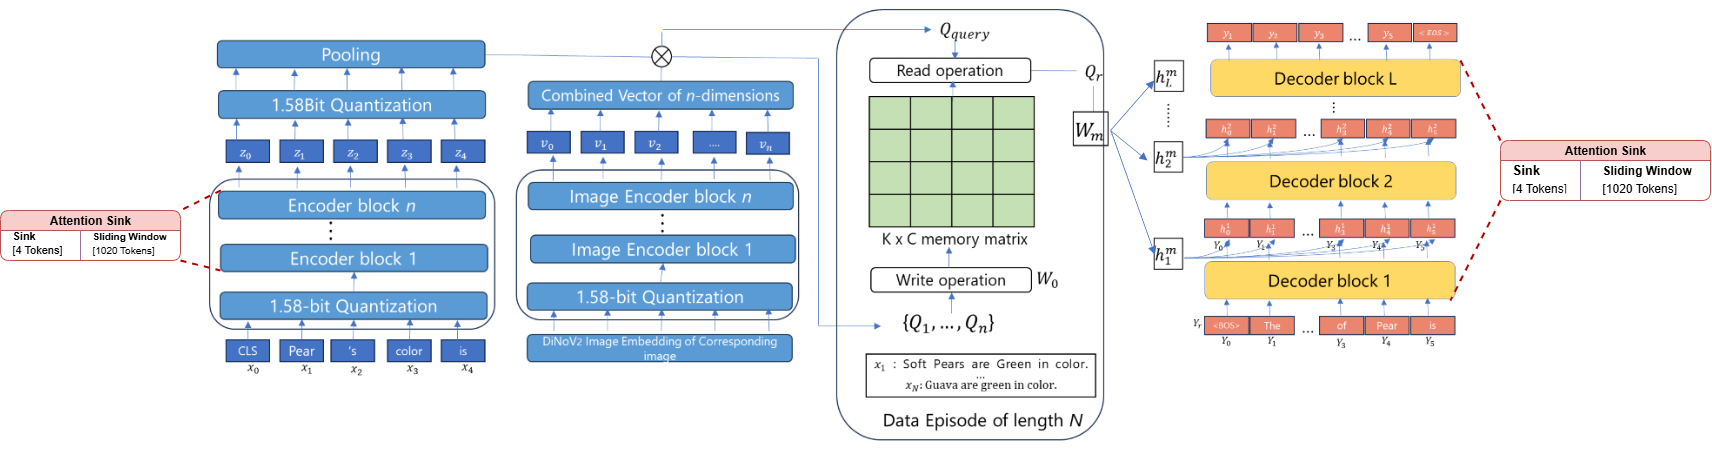
\includegraphics[width=\textwidth]{FIG/BitMar-Architecture.png}
% 	\caption{BitMar Architecture: $X$ and $X_{query}$ represent multimodal episode inputs - text tokens and corresponding DiNOv2-compressed image features. Quantized representations ($z$ and $v$) are computed via BitNet 1.58-bit quantized encoders for both text and vision branches, those encodings are pooled and fused into $Q$ and $Q_{query}$ using cross-modal attention. Attention sinks with a sliding window mechanism (4 sink tokens + 1020 window tokens) enable infinite context processing in both encoder and decoder blocks. A fixed-size $K \times C$ episodic memory matrix stores and retrieves cross-modal episode vectors with quantized read and write weights $(W, W_0)$, supporting SD card-based offloading for edge deployment.}
% 	\label{fig:bitmar}
% \end{figure*}

% We propose BitMar, a deployable, quantized multimodal language model designed for efficient image–text generation under resource constraints. The architecture follows a four-stage pipeline: (1) parallel low-bit encoders for text and vision inputs, (2) cross-modal fusion in a unified latent space, (3) context augmentation via an external episodic memory module, and (4) autoregressive decoding conditioned on both the fused representation and retrieved memory signals. The text encoder is a BitNet-based transformer operating at 1.58-bit precision, enabling compact yet expressive language representations. The vision encoder leverages a DiNOv2 backbone followed by quantization-aware compression to produce efficient visual embeddings. Cross-modal interaction is performed through a lightweight attention mechanism that aligns the 768-dimensional latent representations from both modalities. An external, fixed-size episodic memory stores multimodal context vectors from prior inputs and retrieves relevant entries during generation, injecting them into the decoder via per-layer conditioning. This memory-augmented decoder is inspired by Memory-Augmented Neural Networks (MANNs) introduced by~\citep{graves-dynamicexternalmemory-2016}, but diverges in its design by incorporating low-bit quantization and enabling cross-modal memory retrieval. While~\citep{graves-dynamicexternalmemory-2016} used a simple memory module for task-based memory storage and retrieval, BitMar's memory mechanism integrates both text and visual modalities to enhance multimodal generation, allowing for a richer representation of contextual information. The decoder itself is a BitNet-based autoregressive transformer equipped with streaming attention through attention sinks, allowing low-latency, long-context generation.

% \subsection{Text Encoders}
% \textbf{Architecture}. The text encoder is a lightweight, quantized Transformer designed to efficiently process language inputs under strict resource constraints. The architecture consists of four Transformer layers with a hidden dimension $d=128$ and four attention heads $h=4$, supporting sequences of up to 256 tokens. This compact configuration provides a balance between expressiveness and computational efficiency, making it suitable for deployment in low-latency environments.

% \textbf{Quantization}. To further reduce memory footprint and accelerate computation, we apply two levels of quantization:
% \begin{itemize}
%     \item \textbf{Weight Quantization}. All linear projection weights in the multi-head self-attention (MHSA) and feed-forward network (FFN) submodules are quantized to ternary values $\{-1,0,+1\}$ using learned per-layer scaling factors. This scheme corresponds to 1.58-bit quantization, where the scale parameter is trained jointly with the network parameters, allowing each layer to adapt its effective dynamic range.
%     \item \textbf{Activation Quantization}. Token-wise activations are quantized to 8 bits using per-token max-abs scaling. For each token embedding vector, we compute its maximum absolute value across dimensions and use it to scale the vector into the $[-127,127]$ integer range before discretization. This localized scaling preserves fine-grained detail for each token, mitigating the information loss often observed in global scaling methods.
% \end{itemize}

% This dual quantization strategy substantially reduces the model’s memory and compute requirements, while the combination of ultra-low-bit weights and 8-bit activations ensures stable training and inference.

% \textbf{Attention Sinks Injection}. To enable efficient processing of long or streaming sequences without quadratic growth in memory usage, we incorporate attention sinks into every self-attention layer. Let $S$ denote the number of sink tokens and $W$ the sliding-window size. During encoding, we maintain a key–value ($KV$) cache containing:

% \begin{itemize}
%     \item The first $S=4$ sink tokens, which are never evicted, serving as persistent global context anchors.
%     \item The most recent $W=1,020$ tokens, stored in a sliding window.
% \end{itemize}

% When a new token arrives, the cache evicts the oldest token in the window, merges the sink tokens with the updated window tokens, and clamps positional embeddings to the range $[0,S+W-1]$. This ensures that the model’s positional encoding space remains consistent despite the shifting window. The merged sink–window set is then used in the self-attention computation, enabling seamless attention over arbitrarily long contexts with fixed memory usage. This combination of low-bit quantization and streaming attention mechanisms allows the text encoder to operate effectively in constrained environments, maintaining high throughput while preserving long-range dependencies.

% \subsection{Vision Encoders}
% The vision encoder leverages pretrained DiNOv2 representations to provide high-quality visual features while avoiding the computational cost of full backbone inference during training and deployment. Specifically, 768-dimensional patch-level features are extracted offline for each image using a frozen DiNOv2 backbone~\citep{oquab-dinov2-2024}. This setup enables the model to operate without GPU-intensive convolutional or transformer vision stacks at inference time, reducing the overall system complexity.

% \textbf{Spatial Pooling}.
% Before compression, we apply 2×2 average pooling to the patch grid, reducing the total patch count by a factor of four. This operation decreases the token sequence length in subsequent processing while retaining coarse spatial structure. The pooled feature map maintains the same 768-dimensional embedding per patch.

% \textbf{Compression Module}.
% To align with the text encoder’s compact representation space and minimize memory footprint, we employ a learned two-layer MLP bottleneck to compress the 768-dimensional DiNOv2 features to a 128-dimensional latent vector. The transformation proceeds as:

% \vspace{-1.5em}
% \begin{align}
%     \mathbf{z}^{(1)}_{\text{vis}} &= \mathrm{ReLU}(\mathbf{W}_1 \mathbf{x}_{\text{vis}} + \mathbf{b}_1), \\
%     \mathbf{z}^{(2)}_{\text{vis}} &= \mathbf{W}_2 \mathbf{z}^{(1)}_{\text{vis}} + \mathbf{b}_2
% \end{align}
% \vspace{-1.5em}

% where $\mathbf{W}_1 \in \mathbb{R}^{384\times768}$, $\mathbf{W}_2 \in \mathbb{R}^{128\times384}$, and dropout is applied after the ReLU activation for regularization.

% \subsection{Cross-Modal Fusion}
% The cross-modal fusion module aligns and integrates the latent representations from the text and vision encoders into a unified multimodal representation. The module operates on pooled token embeddings from each modality: the text encoder output $ \mathbf{Z} \in \mathbb{R}^{n \times 128} $ and the vision encoder output $ \mathbf{V} \in \mathbb{R}^{n \times 128} $, where $n$ denotes the token length after pooling or spatial reduction.

% \textbf{Fusion Mechanism}.
% We adopt a standard cross-attention mechanism in which the text tokens act as the queries $(Q)$ and the vision tokens serve as the keys $(K)$ and values $(V)$. This design allows the text representation to selectively attend to relevant visual information, aligning semantic content in the text with spatial and object-level cues in the image features. The attention weights are computed as:

% \vspace{-1.5em}
% \begin{equation}
%     \mathrm{Attention}(Q, K, V) = 
%     \mathrm{softmax}\left( \frac{QK^\top}{\sqrt{d_k}} \right) V
% \end{equation}
% \vspace{-1.5em}

% where $d_k$ is the key dimensionality.

% \textbf{Quantization Strategy}.
% To maintain the model’s low-bit efficiency, all projection matrices used in generating $Q, K,V$ and the fused output are quantized to 1.58 bits using ternary weights $\{-1,0,+1\}$ with learned per-layer scaling factors. The softmax computation and the residual add–layer normalization operations are performed in FP32 to preserve numerical stability and avoid accumulation errors during attention score computation.

% The result of the cross-attention operation is the fused representation $ \mathbf{F} \in \mathbb{R}^{n \times 128} $ , where each text token embedding has been enriched with complementary visual information. To prepare this multimodal representation for interaction with the episodic memory module, we apply either mean pooling or a learned pooling operation over the sequence dimension to produce a single query matrix $ \mathbf{Q_{query}} \in \mathbb{R}^{n \times 128} $. This query matrix is subsequently used to retrieve relevant context vectors from the episodic memory, ensuring that the decoder is conditioned on both the current multimodal input and relevant prior experiences.

% \subsection{Episodic Memory}
% The episodic memory module augments the fused multimodal representation with contextual information stored across prior inference steps. The memory is implemented as a learnable matrix $ \mathbf{M} \in \mathbb{R}^{K \times C} $, with $K=512$ slots and embedding dimensionality $C=128$, where each slot stores a latent vector that summarizes the multimodal context from past inputs. After experimentation, we found that 512 memory slots provided a more effective capture of the latent space, resulting in improved contextual recall and memory utilization during decoding.

% \textbf{Writing}.
% At each generation step $ t \in [[1,n]] $, the current episodic query vector $ \mathbf{Q_{query,t}} \in \mathbb{R}^{C} $ is written into the memory via learned write weights $ \mathbf{W_{w}} \in \mathbb{R}^{K} $. The update rule is as follows:

% \vspace{-1em}
% \begin{equation}
% \mathbf{M} \leftarrow \mathbf{M} + \alpha \cdot \mathbf{W}w^\top \mathbf{Q}_{query,t}
% \end{equation}
% \vspace{-1.5em}

% where $\alpha=0.2$ is a fixed update rate controlling the influence of new entries. This formulation enables soft writing to multiple memory slots in proportion to $W_w$, rather than hard assignment to a single slot.

% \textbf{Reading}.
% To retrieve relevant context, we compute read weights using content-based addressing:

% \vspace{-1em}
% \begin{equation}
% \mathbf{W}r = \mathrm{softmax}(\mathbf{M} \mathbf{Q}_{query})
% \end{equation}
% \vspace{-1.5em}

% where the similarity between $Q_{query}$ and each memory slot determines its contribution. The retrieved memory vector is then:

% \vspace{-1em}
% \begin{equation}
% \mathbf{M}_r = \mathbf{W}_r^\top \mathbf{M} \in \mathbb{R}^{1 \times C}
% \end{equation}
% \vspace{-1.5em}

% which is concatenated or added to the fused multimodal representation before decoding.

% \textbf{External Storage}.
% For long-running sessions or deployment on memory-constrained devices, the memory matrix $M$ can be offloaded to external storage (e.g., an SD card) via a Python utility that saves and loads memory tensors without gradient tracking. This allows a persistent state between sessions without increasing runtime GPU memory usage.

% \textbf{Regularization}.
% To prevent drift and ensure stability, we apply an $\ell_2$ penalty to memory updates:

% \vspace{-1em}
% \[
% \mathcal{L}_{\text{mem}} = \lambda \|\Delta \mathbf{M}\|_2^2
% \]
% \vspace{-1.5em}

% Additionally, a usage-based forgetting mechanism gradually attenuates the contribution of slots that have not been accessed recently, ensuring that the memory remains relevant to the current context while preventing unbounded growth of stale information.


% \subsubsection{Decoder with Attention Sinks}
% The decoder is a lightweight, autoregressive transformer that generates text conditioned on both the current multimodal context and retrieved episodic memory signals. The architecture comprises four causal transformer layers, each with a hidden dimension of 128, four attention heads, and a maximum generation length of 256 tokens.

% \textbf{Attention Sinks for Long-Context Generation}.
% To support generation over sequences longer than the maximum length without quadratic growth in attention computation, we integrate attention sinks into every decoder self-attention layer. Each layer maintains a key–value $(KV)$ cache consisting of:~\textbf{Sink tokens}. The first $S$ tokens (persistent anchors) are never evicted, providing a stable global context.
% \textbf{Sliding window}. The most recent $W$ tokens that capture local dependencies.


% For each new token, the window cache evicts the oldest entry, merges with the sink tokens, and clamps positional indices to the range $[0, S + W - 1]$. This mechanism ensures consistent positional encoding and enables the decoder to attend to arbitrarily long contexts while keeping memory usage bounded.

% \textbf{Memory Integration}.
% At each decoding step, the retrieved memory vector $ \mathbf{M_{r}} \in \mathbb{R}^{1 \times 128} $ from the episodic memory module is projected through a learnable linear layer and then combined with the token input embeddings for the current step. The integration can be implemented in two ways:~\textbf{Concatenation}. $[x_{t}; M_{r}]$ is passed through a projection layer to match the decoder’s hidden size.
% \textbf{Addition}. $M_{r}$ is added directly to the input embedding $x_{t}$ as a residual conditioning signal. This conditioning allows the decoder to leverage both the current fused multimodal context and relevant episodic knowledge during text generation.

% \textbf{Output Projection}.
% The decoder’s final hidden states are mapped to vocabulary logits via a BitNet-quantized linear layer BitNetLinear (128 $\rightarrow$ 50,257), corresponding to the GPT-2 vocabulary size. While the projection weights are quantized for efficiency, the logits are computed in FP32 to preserve numerical stability in the subsequent softmax cross-entropy loss computation.

% \subsubsection{Training Objectives}
% The model is trained using a multi-objective loss function that combines generation, cross-modal alignment, and memory stability components.

% \textbf{Language Modeling Loss}.
% The primary objective is a language modeling loss $\mathcal{L}_{\text{lm}}$, implemented as the token-level cross-entropy between the decoder’s predicted probability distribution and the ground-truth caption tokens. At each decoding step $t$, the loss is:

% \vspace{-1.5em}
% \begin{equation}
% \mathcal{L}_{\text{lm}} = - \frac{1}{T} \sum_{t=1}^T \log p_{\theta}(y_t^\ast \mid y_{<t}, \mathbf{X})
% \end{equation}
% %\vspace{-1.5em}

% where $T$ is the target length, $y_t^\ast$ is the gold token at step $t$, and $X$ denotes the fused multimodal input. This term has a fixed weight of 1.0 in the total loss.

% \textbf{Cross-Modal Contrastive Loss}.
% To enforce alignment between modalities, we introduce a cross-modal contrastive loss $\mathcal{L}_{\text{cm}}$ following an InfoNCE formulation~\citep{oord_representation_2018}. Given a batch of paired text embeddings $z_{t}$ and vision embeddings $z_{v}$,  we compute cosine similarities for all pairs in the batch and apply a softmax over negative pairs:

% %\vspace{-1.5em}
% \small
% \begin{equation}
% \mathcal{L}{\text{cm}} = - \frac{1}{N} \sum_{i=1}^N \log \frac{\exp(\mathrm{sim}(\mathit{z}_t^i, \mathit{z}_v^i) / \tau)}{\sum{j=1}^N \exp(\mathrm{sim}(\mathit{z}_t^i, \mathit{z}_v^j) / \tau)}
% \end{equation}
% \normalsize
% %\vspace{-1.5em}

% where $\mathrm{sim}(\cdot, \cdot)$ denotes cosine similarity, $\tau$  is a temperature parameter, and $N$  is the batch size. This loss is applied symmetrically for both text-to-vision and vision-to-text retrieval and is weighted by 1.5.

% \textbf{Memory Consistency Loss}.
% To ensure stability in the episodic memory module, we introduce a memory consistency loss $\mathcal{L}_{\text{mem}}$, defined as the $\ell_2$ distance between consecutive memory write vectors:

% \vspace{-1.5em}
% \begin{equation}
% \mathcal{L}_{\text{mem}} = | \mathbf{M}^{(t)}_{\text{write}} - \mathbf{M}^{(t-1)}_{\text{write}} |_2^2
% \end{equation}
% %\vspace{-1.5em}

% This term discourages abrupt changes in stored memory representations and is weighted by 0.1.

% \textbf{Total Objective}.
% The final training objective is a weighted sum of the three components:

% %\vspace{-1.5em}
% \begin{equation}
% \mathcal{L} = \mathcal{L}_{\text{lm}} + 1.5 , \mathcal{L}_{\text{cm}} + 0.1 , \mathcal{L}_{\text{mem}}
% \end{equation}
% %\vspace{-1.5em}

% This formulation balances caption generation accuracy, cross-modal representation alignment, and stability in the episodic memory over time.

% \subsubsection{Adaptive Training Controller}
% To maintain stable multimodal alignment and mitigate the risk of modality collapse during training, we introduce an Adaptive Training Controller (ATC) that dynamically adjusts the optimization process based on online monitoring of cross-modal alignment metrics.

% \textbf{Monitoring Phase}.
% The ATC continuously tracks the exponential moving average (EMA) of the cross-modal cosine similarity between pooled text and vision embeddings. The EMA is computed over a rolling window of 200 training steps, providing a smoothed estimate of alignment trends while reducing the impact of short-term fluctuations.

% \textbf{Intervention Trigger}.
% An intervention is triggered if the EMA exhibits a relative drop greater than 0.12 compared to its recent maximum value and if at least 800 steps have elapsed since the last intervention. This dual criterion ensures that adjustments are applied only when there is a sustained and significant degradation in alignment, avoiding overreaction to minor noise.

% \textbf{Intervention Actions}.
% Upon triggering, the ATC randomly selects one of the following stabilization actions:
% \begin{itemize}
%     \item Freeze text encoder — temporarily halts updates to all parameters in the text encoder.
%     \item Freeze vision encoder — temporarily halts updates to all parameters in the vision encoder.
%     \item Boost cross-modal loss weight — increases the weight of the cross-modal contrastive loss $\mathcal{L}_{\text{cm}}$ to strengthen alignment learning.
% \end{itemize}

% The selected action is applied for a freeze duration of 1,500 training steps, during which the chosen component remains fixed or the loss weight remains boosted.

% \textbf{Stability Benefits}.
% By adaptively freezing one modality or emphasizing cross-modal supervision, the ATC prevents modality collapse, a failure mode where one encoder dominates the shared representation space, leading to degraded cross-modal retrieval and generation quality. This mechanism ensures that both encoders contribute meaningfully throughout training and that alignment remains stable even under challenging optimization conditions.

\section{Method}
\label{sec:method}

\begin{figure*}[t]
    \centering
    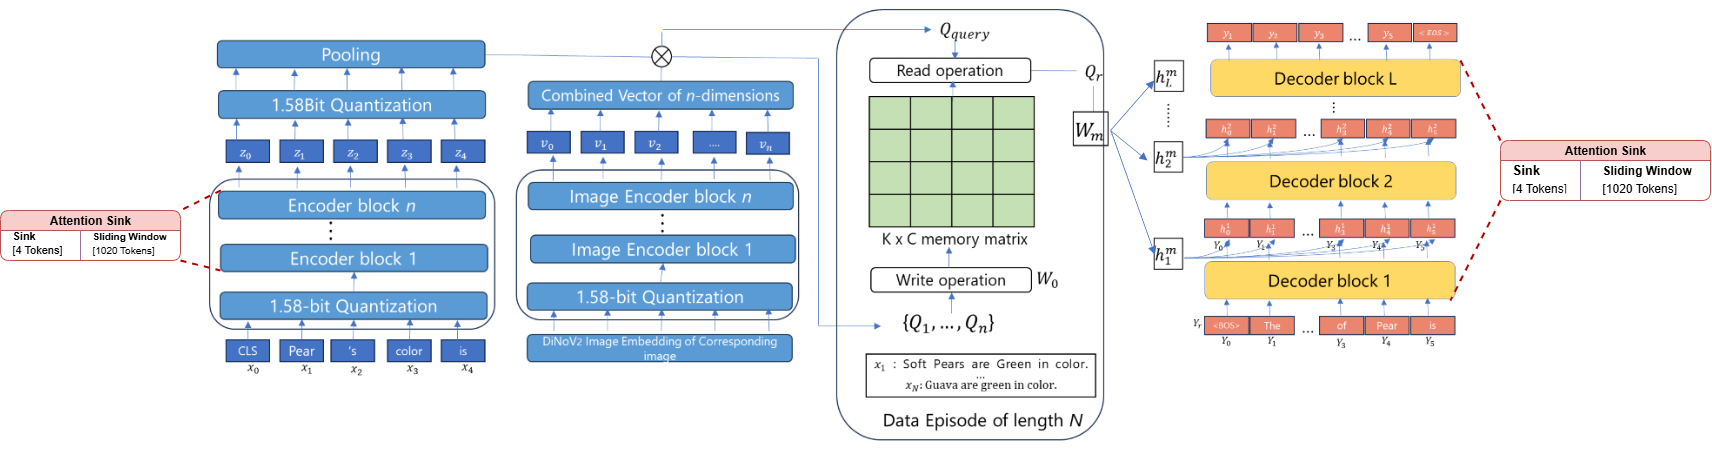
\includegraphics[width=\textwidth]{FIG/BitMar-Architecture.png}
    \caption{\textbf{BitMar Architecture.}
    The model processes multimodal inputs: text tokens and DiNOv2-compressed image features.
    Quantized encoders (1.58-bit) generate compact text and vision embeddings ($z$, $v$), which are fused via cross-modal attention into shared query representations ($Q$, $Q_{query}$).
    A sliding-window attention mechanism enables long-context processing.
    A fixed episodic memory matrix ($K \times C$) stores and retrieves multimodal context vectors through quantized read/write weights ($W$, $W_0$), supporting optional SD-card offloading for edge deployment.
    }
    % \caption{BitMar Architecture. $X$/$X_{query}$: multimodal inputs (text tokens + DiNOv2-compressed image features). Quantized encoders produce $z$/$v$ (1.58-bit). Cross-modal attention pools/fuses to $Q$/$Q_{query}$. Attention sinks with a sliding window (4 sink tokens, 1020 window) enable infinite-context processing. A fixed $K\times C$ episodic memory stores/retrieves episode vectors with quantized read/write weights $(W,W_0)$, supporting SD-card offloading.}
    \label{fig:bitmar}
\end{figure*}

We introduce \textbf{BitMar}, a deployable quantized multimodal LM for efficient image–text generation under tight resources. The four-stage pipeline is: 
(1) \textbf{parallel low-bit text/vision encoders}; 
(2) \textbf{cross-modal fusion} in a shared latent space; 
(3) \textbf{context augmentation} via external episodic memory; 
(4) \textbf{autoregressive decoding} conditioned on fused and retrieved signals. 
Text uses a BitNet transformer at 1.58-bit precision; vision uses DiNOv2 features plus quantization-aware compression. Fusion aligns 768-D modality latents via lightweight attention. A fixed-size episodic memory stores prior multimodal contexts and injects retrieved vectors into the decoder per layer. Unlike classic MANNs~\citep{graves-dynamicexternalmemory-2016}, BitMar integrates cross-modal retrieval under low-bit constraints. The decoder is a BitNet-based autoregressive transformer with streaming attention via attention sinks for low-latency, long-context generation.

% We present \textbf{BitMar}, a deployable quantized multimodal language model designed for efficient image–text generation under strict resource constraints. 
% The proposed architecture follows a four-stage pipeline: 
% (1) \textbf{parallel low-bit text and vision encoders} for compact representation learning; 
% (2) \textbf{cross-modal fusion} within a shared latent space to align textual and visual features; 
% (3) \textbf{context augmentation} through an external episodic memory that stores and retrieves multimodal context vectors; and 
% (4) \textbf{autoregressive decoding} conditioned on both fused embeddings and retrieved memory signals. 
% The text encoder adopts a 1.58-bit BitNet transformer, while the vision branch employs DiNOv2 features with quantization-aware compression. 
% Fusion aligns the 768-dimensional modality representations via lightweight attention. 
% A fixed-size episodic memory maintains previous multimodal contexts and injects the retrieved vectors into each decoder layer. 
% Unlike conventional memory-augmented neural networks~\citep{graves-dynamicexternalmemory-2016}, BitMar performs cross-modal retrieval under low-bit constraints, enabling a BitNet-based autoregressive decoder with streaming attention via attention sinks for low-latency, long-context generation.


\subsection{Text Encoders}


\textbf{Architecture.} A 4-layer quantized Transformer ($d{=}128$, $h{=}4$) supports up to 256 tokens, balancing expressiveness and efficiency.

\textbf{Quantization.} 
\emph{Weights:} all MHSA/FFN projections use ternary $\{-1,0,+1\}$ with learned per-layer scales (1.58-bit). 
\emph{Activations:} token-wise 8-bit using per-token max-abs scaling to $[-127,127]$, preserving local detail and stable training/inference.

\textbf{Attention sinks (streaming).} With $S{=}4$ sink tokens (never evicted) and window $W{=}1020$, the KV cache maintains persistent anchors + recent tokens. On each new token, the oldest in-window token is evicted; sink and window sets are merged; positions are clamped to $[0,S{+}W{-}1]$. This yields fixed-memory, long-context attention under low-bit compute.

\subsection{Vision Encoders}
We use frozen DiNOv2~\citep{oquab-dinov2-2024} to extract 768-D patch features offline, avoiding heavy vision backbones at inference. $2{\times}2$ average pooling reduces the number of patches $4{\times}$ while keeping 768-D per patch. 2-layer MLP bottleneck then compresses 768$\rightarrow$128 with ReLU and dropout between layers (parameters $\mathbf{W_1}\in\mathbb{R}^{384\times 768}, \mathbf{W_2}\in\mathbb{R}^{128\times 384}$), all subsequent fusion/memory/decoder paths operate in 128-D.

% \textbf{Spatial pooling.} $2{\times}2$ average pooling reduces patches $4{\times}$ while keeping 768-D per patch.

% \textbf{Compression.} A 2-layer MLP bottleneck maps 768$\rightarrow$128:
% \begin{align}
%     \mathbf{z}^{(1)}_{\text{vis}} &= \mathrm{ReLU}(\mathbf{W}_1 \mathbf{x}_{\text{vis}} + \mathbf{b}_1), \\
%     \mathbf{z}^{(2)}_{\text{vis}} &= \mathbf{W}_2 \mathbf{z}^{(1)}_{\text{vis}} + \mathbf{b}_2
% \end{align}
% with dropout after ReLU.

\subsection{Cross-Modal Fusion}
Given pooled text tokens $\mathbf{Z}\in\mathbb{R}^{n_t\times128}$ and vision tokens
$\mathbf{V}_{\text{img}}\in\mathbb{R}^{n_v\times128}$, we apply standard cross-attention~\citep{vaswani2017attention}
(text queries, vision keys/values; cf.\ Transformer attention) to obtain the fused
sequence $\mathbf{F}\in\mathbb{R}^{n_t\times128}$. All $Q/K/V$ and fusion projections
use 1.58-bit ternary weights with learned scales; softmax and residual/LN are in FP32.
We then pool $\mathbf{F}$ (mean or learned) to a single vector
$\mathbf{q}_{\text{mem}}\in\mathbb{R}^{128}$ to query episodic memory.

% Given pooled outputs $\mathbf{Z}\in\mathbb{R}^{n\times128}$ (text) and $\mathbf{V}\in\mathbb{R}^{n\times128}$ (vision), we apply cross-attention with text queries and vision keys/values:
% \begin{equation}
%     \mathrm{Attention}(Q,K,V)=\mathrm{softmax}\!\left(\frac{QK^\top}{\sqrt{d_k}}\right)V
% \end{equation}
% All projections for $Q,K,V$ and the fused output use 1.58-bit ternary weights with learned scales; softmax and residual/LN run in FP32. The fused sequence $\mathbf{F}\in\mathbb{R}^{n\times128}$ is pooled (mean or learned) to form $\mathbf{Q_{query}}\in\mathbb{R}^{n\times128}$ for memory retrieval.

\subsection{Episodic Memory}

We maintain a learnable matrix $\mathbf{M}\in\mathbb{R}^{K\times C}$ (default $K{=}512$, $C{=}128$) that stores multimodal episode vectors.

\paragraph{Writing.}
At step $t$, we compute a pooled query $\mathbf{q}_t\in\mathbb{R}^{C}$ and learned write weights $\mathbf{W}_w\in\mathbb{R}^{K}$. We perform soft multi-slot writes with rate $\alpha{=}0.2$ via an outer product:
\begin{equation}
\mathbf{M} \leftarrow \mathbf{M} + \alpha\, \mathbf{W}_w \,\mathbf{q}_t^{\top}.
\label{eq:mem_write}
\end{equation}

\paragraph{Reading.}
We use content-based addressing \citep{graves-dynamicexternalmemory-2016}:
\begin{equation}
\begin{aligned}
\mathbf{W}_r &= \operatorname{softmax}(\mathbf{M}\,\mathbf{q}_t)\in\mathbb{R}^{K},\\
\mathbf{M}_r &= \mathbf{W}_r^{\top}\mathbf{M}\in\mathbb{R}^{1\times C}.
\end{aligned}
\label{eq:mem_read}
\end{equation}

\paragraph{Regularization.}
To avoid thrashing, we penalize abrupt updates to the store with a Frobenius penalty,
% \begin{equation}
$
\mathcal{L}_{\mathrm{reg}} = \lambda \,\big\lVert \Delta\mathbf{M}\big\rVert_{F}^{2},
\quad
\Delta\mathbf{M} := \mathbf{M}^{(t)} - \mathbf{M}^{(t-1)}.
\label{eq:mem_reg}
$
% \end{equation}
We additionally apply usage-based forgetting to down-weight stale slots.
% A learnable matrix $\mathbf{M}\in\mathbb{R}^{K\times C}$ ($K{=}512$, $C{=}128$) stores multimodal episode vectors; 512 slots worked best empirically.

% \textbf{Writing.} For step $t\in[[1,n]]$, write with learned weights $\mathbf{W_w}\in\mathbb{R}^K$:
% \begin{equation}
% \mathbf{M} \leftarrow \mathbf{M} + \alpha \cdot \mathbf{W}w^\top \mathbf{Q}_{\text{query},t}
% \end{equation}
% with update rate $\alpha{=}0.2$ (soft multi-slot writes).

% \textbf{Reading.} Content addressing:
% \begin{equation}
% \mathbf{W}r = \mathrm{softmax}(\mathbf{M}\mathbf{Q}_{\text{query}})
% \end{equation}
% and retrieved vector
% \begin{equation}
% \mathbf{M}_r = \mathbf{W}_r^\top \mathbf{M}\in\mathbb{R}^{1\times C}.
% \end{equation}

% \textbf{External storage.} $\mathbf{M}$ can be offloaded (e.g., external SD card) to persist state without GPU memory growth.

% \textbf{Regularization.} We penalize updates with
% \[
% \mathcal{L}_{\text{reg}}=\lambda\|\Delta\mathbf{M}\|_2^2
% \]
% and apply usage-based forgetting to down-weight stale slots.

\subsubsection{Decoder with Attention Sinks}
A 4-layer causal Transformer ($d{=}128$, $h{=}4$, max length 256) conditions on fused inputs and retrieved memory.

\textbf{Long-context generation.} Each layer, similarly as the text encoder, maintains KV caches of $S$ sink tokens and a window of $W$ recent tokens.

\textbf{Memory integration.} $\mathbf{M_r}\in\mathbb{R}^{1\times128}$ is projected and combined with token embeddings via either concatenation $[x_t;\mathbf{M_r}]$ (then projected) or residual addition $x_t{+}\mathbf{M_r}$.

\textbf{Output projection.} BitNet-quantized linear layer (128$\rightarrow$50{,}257) maps to GPT-2 vocab logits; logits computed in FP32.

\subsubsection{Training Objectives}
We complement standard Language Modeling cross-entropy~\citep{vaswani2017attention} and an InfoNCE cross-modal~\citep{oord_representation_2018} term with a memory-consistency regularizer~\autoref{eq:memory_consistent} that penalizes changes between successive writes to the episodic store, which discourages oscillatory updates and helps retain slot semantics. The total loss integrates these factors as~\autoref{eq:total_obj}. We set $\mathcal{L}_{\text{cm}}=1.5$ to prioritize cross-modal alignment, and $\mathcal{L}_{\text{mem}}=0.1$ as a light stabilizer.
% \textbf{Language modeling.} We optimize a composite objective with three terms. First, we use standard token-level cross-entropy for language modeling~\citep{vaswani2017attention}. Second, we align pooled text/vision embeddings with an InfoNCE cross-modal contrastive objective~\citep{oord_representation_2018}. Third, we complement a memory-consistency penalty~\autoref{eq:memory_consistent}. Lastly, we compute the total loss as a weighted sum~\autoref{eq:total_obj}:
% \begin{equation}
% \mathcal{L}_{\text{lm}} = - \frac{1}{T} \sum_{t=1}^T \log p_{\theta}(y_t^\ast \mid y_{<t}, \mathbf{X})
% \end{equation}

% \textbf{Cross-modal contrastive (InfoNCE)~\citep{oord_representation_2018}}
% \small
% \begin{equation}
% \mathcal{L}_{\text{cm}} = - \frac{1}{N} \sum_{i=1}^N \log \frac{\exp(\mathrm{sim}(\mathit{z}_t^i, \mathit{z}_v^i) / \tau)}{\sum_{j=1}^N \exp(\mathrm{sim}(\mathit{z}_t^i, \mathit{z}_v^j) / \tau)}
% \end{equation}
% \normalsize

\textbf{Memory consistency.}
\begin{equation}
\mathcal{L}_{\text{mem}} = | \mathbf{M}^{(t)}_{\text{write}} - \mathbf{M}^{(t-1)}_{\text{write}} |_2^2
\label{eq:memory_consistent}
\end{equation}

\textbf{Total objective.}
\begin{equation}
\mathcal{L} = \mathcal{L}_{\text{lm}} + 1.5 · \mathcal{L}_{\text{cm}} + 0.1 · \mathcal{L}_{\text{mem}}
\label{eq:total_obj}
\end{equation}

% \subsubsection{Adaptive Training Controller}
% We stabilize alignment via an \textbf{Adaptive Training Controller (ATC)} that monitors the exponential moving average (EMA) of cross-modal cosine similarity over a 200-step window.

% \textbf{Trigger.} Intervene on a relative EMA drop $>0.12$, from the recent maximum and, if $\geq$800 steps since the last intervention.

% \textbf{Actions.} Randomly: freeze text encoder; freeze vision encoder; or boost the weight of $\mathcal{L}_{\text{cm}}$. The chosen action persists for 1{,}500 steps.

% \textbf{Effect.} ATC mitigates modality collapse by enforcing balanced contributions to the shared space and maintaining retrieval/generation quality under challenging optimization.

\textbf{Adaptive Training Controller.} When a 200-step EMA of cross-modal cosine similarity drops by $>0.12$ from its recent max (with an $\geq$800-step cooldown), we randomly freeze one encoder or upweight $\mathcal{L}_{\text{cm}}$ for 1,500 steps to prevent modality collapse.












% \section{Experimental Setup}
% \label{sec:exp}

% We formulate four questions that reflect the evidence we present: (1) Can a 14M, 1.58-bit BitMar deliver usable accuracy compared to compact/low-bit baselines~\autoref{tab:ranking_metrics}? (2) Where does it excel or lag in language and multimodal tasks~\autoref{tab:bitmar_babylm_results}? (3) Does episodic memory evolve from diffuse to structured activations indicative of learned retrieval~\autoref{fig:heatmap_comparison}? (4) Does quantization/compression effectiveness improve over training under extreme low-bit constraints~\autoref{fig:quantization}?

% \subsection{Dataset}
% Our training corpus comprises 100 million tokens, evenly divided between multimodal caption data and text-only data.

% \textbf{Multimodal Captions (50M tokens)}.
% The multimodal portion is constructed from Conceptual Captions (CC3M)~\citep{sharma-CC3M-2018} and Localized Narratives dataset~\citep{ponttuset-localized-narratives-2020}, providing high-quality image–text pairs. Each caption is perfectly aligned with precomputed DiNOv2 visual features, ensuring consistent visual–linguistic correspondence. Visual features are extracted once using a frozen DiNOv2 backbone and stored for reuse during training, eliminating the need for online vision encoding.

% \textbf{Text-Only Data (50M tokens)}.
% The text-only portion is derived from the BabyLM~\citep{Charpentier-babylm-2025} split, covering six domains: BNC Spoken, CHILDES, Gutenberg, OpenSubtitles, Simple English Wikipedia, and Switchboard. This diversity provides exposure to a range of linguistic registers, from conversational to literary and encyclopedic texts.

% \textbf{Mixture and Hold-out}.
% The final training mixture is uniformly sampled at a 50:50 ratio between multimodal and text-only sources. No dedicated validation split is used; instead, a 1M-token hold-out set is maintained to monitor cross-modal alignment (via cosine similarity metrics) and language modeling perplexity throughout training. This setup enables continual performance tracking without interrupting training for separate evaluation runs.

% \textbf{Preprocessing}.
% Text data is tokenized using the GPT-2 byte pair encoding tokenizer, with a maximum sequence length of 256 tokens. Sequences exceeding this limit are truncated, and shorter sequences are padded to maintain batch uniformity. Visual features are stored in memory-mapped "\texttt{.npy}" files and loaded with on-the-fly compression, reducing I/O overhead and memory usage while maintaining high throughput during multimodal batching.

% \subsection{Training Configuration}
% All experiments are conducted on a compute cluster equipped with 8× NVIDIA A100 GPUs. We use mixed-precision (FP16) training to reduce memory usage and accelerate computation, combined with gradient checkpointing to further lower the memory footprint in long-context training.

% \textbf{Batching}. 
% Each training step processes 64 sequences per batch, with an effective batch size of 128 achieved via gradient accumulation over 2 steps. This configuration balances GPU memory constraints with stable gradient estimates.

% \textbf{Optimization}. 
% We train the model using AdamW8bit $2 \times 10^{-4}$~\citep{ilya-sgdr-2016}, with parameters $T_0=1,000$ (initial cycle length), $T_{mult}=2$ (cycle length multiplier), and a minimum learning rate $\eta_{min}=0.1 \times lr$. We train for up to 10 epochs, without early stopping based on token count, ensuring consistent exposure to the entire dataset mixture in each epoch. The cosine-with-restarts scheduler allows the learning rate to decay smoothly within each cycle before restarting, helping the model escape shallow local minima and potentially improving generalization.

% We use Weights and Biases for experiment tracking, logging every 500 steps: Primary and auxiliary loss values ($\mathcal{L}_{\text{lm}}$, $\mathcal{L}_{\text{cm}}$, $\mathcal{L}_{\text{mem}}$), Cross-modal alignment metrics, Episodic memory usage statistics, Attention maps and memory retrieval visualizations, FLOPs per step for efficiency analysis. This monitoring setup enables both quantitative tracking and qualitative inspection of the model’s behavior over training.

% \subsection{Hyperparameters}
% Table \ref{tab:hyperparams} lists the key architectural and training hyperparameters used in all experiments. The configuration reflects a trade-off between model expressiveness and efficiency, making it suitable for deployment in constrained environments. The text and vision latent dimensions are both set to 128, ensuring that cross-modal fusion can be performed without expensive projection layers. The 4-layer text encoder combined with a relatively small memory size (512 slots × 128 dimensions) keeps the computational footprint low while retaining the capacity to store and retrieve relevant context. The number of memory slots was determined experimentally, and 512 slots were found to provide optimal performance in capturing the latent space and improving episodic recall efficiency, as compared to using fewer slots.

% For long-context modeling, the attention sink size (4) and sliding window size (1,020) enable the decoder to attend to persistent global anchors and recent tokens without unbounded memory growth. The cross-modal loss weight (1.5) biases optimization toward strong vision-language alignment, while the memory consistency weight (0.1) helps stabilize the episodic memory by penalizing significant updates. The adaptive training controller thresholds, including the drop threshold of 0.12, freeze duration of 1,500 steps, and minimum 800 steps between interventions, are tuned to prevent modality collapse while minimizing the frequency of disruptive interventions.

% This combination of hyperparameters yields a model that maintains stable multimodal alignment, supports long-context generation, and operates efficiently within the target hardware constraints.

% \begin{table}[ht]
% \centering
% \small
% \begin{tabular}{l l}
% \hline
% \textbf{Hyperparameter} & \textbf{Value} \\
% \hline
% Text Encoder layers         & 4 \\
% Text hidden dim             & 128 \\
% Memory slots                & 512 \\
% Memory dim                  & 128 \\
% Sink size                   & 4 \\
% Window size                 & 1,020 \\
% Cross-modal loss weight     & 1.5 \\
% Memory consistency weight   & 0.1 \\
% Drop threshold (adaptive)   & 0.12 \\
% Freeze duration (steps)     & 1,500 \\
% Min steps per intervention  & 800 \\
% \hline
% \end{tabular}
% \caption{Training hyperparameters for all experiments.}
% \label{tab:hyperparams}
% \end{table}

% \subsection{Benchmarks and baselines}
% For evaluation, we benchmarked BitMar-14M across six widely used language understanding tasks—ARC-Easy, BoolQ, HellaSwag, WinoGrande, CommonsenseQA, and MMLU—to assess reasoning, commonsense, and factual knowledge under extreme quantization constraints. All experiments used the GPT-2 tokenizer with a maximum sequence length of 256 tokens, and multimodal inputs were aligned with precomputed DiNOv2 vision features. Model outputs were scored using accuracy for each benchmark, with performance compared against a range of baselines including Bonsai 0.5B, OLMo-BitNet 1B, Falcon3-1.58bit 7B, LLaMA3-8B-1.58 8B, and BitNet b1.58 2B. In addition to benchmark accuracy, we monitored the effectiveness of quantization and compression, as well as episodic memory activations throughout training to evaluate representational efficiency and memory utilization. This multi-faceted evaluation setup allowed us to measure not only end-task performance but also the internal dynamics of quantization and memory modules, providing insights into the stability and efficiency of our design.

% \section{Experimental Setup}
% \label{sec:exp}

% We address four questions: (1) Can a 14M, 1.58-bit BitMar achieve usable accuracy vs.\ compact/low-bit baselines (\autoref{tab:ranking_metrics})? (2) Where does it excel or lag across language and multimodal tasks (\autoref{tab:bitmar_babylm_results})? (3) Does episodic memory evolve from diffuse to structured activations (\autoref{fig:heatmap_comparison})? (4) Does quantization effectiveness improve during training (\autoref{fig:quantization})?

\section{Experimental Setup}
\label{sec:exp}

Our experimental framework systematically evaluates the proposed 14M-parameter BitMar model across several critical dimensions. We first benchmark its performance against established compact and low-bit baselines to assess overall viability (\autoref{tab:ranking_metrics}). We then conduct an analysis of its capabilities across a suite of language understanding and multimodal tasks to identify specific strengths and limitations (\autoref{tab:bitmar_babylm_results}). Beyond task performance, we also investigate the internal dynamics of the model, examining how the episodic memory evolves from diffuse to structured activation patterns during training (\autoref{fig:heatmap_comparison}). Finally, we track the progression of quantization efficacy throughout the training process to validate our low-precision approach (\autoref{fig:quantization}).

\subsection{Dataset}
The corpus comprises 100M tokens, split evenly between multimodal captions and text-only data.  

\textbf{Multimodal (50M).} From CC3M~\citep{sharma-CC3M-2018} and Localized Narratives~\citep{ponttuset-localized-narratives-2020}, aligned with precomputed DiNOv2 features (frozen backbone, reused across training).  

\textbf{Text-only (50M).} From BabyLM~\citep{Charpentier-babylm-2025}, spanning six domains (BNC, CHILDES, Gutenberg, OpenSubtitles, Simple English Wikipedia, Switchboard).  

\textbf{Mixture.} Uniform 50:50 sampling; a 1M-token hold-out tracks cross-modal alignment (cosine similarity) and perplexity.  

\textbf{Preprocessing.} GPT-2 BPE tokenizer, max 256 tokens (truncate/pad). Visual features stored as memory-mapped ``.npy'' with on-the-fly compression for efficient batching.

\subsection{Training Configuration}
We trained on an NVIDIA A6000 GPU using FP16 and gradient checkpointing. Each step processed 64 sequences, with two-step gradient accumulation yielding an effective batch size of 128. Optimization used AdamW8bit ($2\!\times\!10^{-4}$) with cosine restarts ($T_0{=}1000$, $T_{\text{mult}}{=}2$, $\eta_{min}{=}0.1lr$) for 10 epochs. We logged to Weights \& Biases every 500 steps, including losses ($\mathcal{L}_{\text{lm}}, \mathcal{L}_{\text{cm}}, \mathcal{L}_{\text{mem}}$), cross-modal alignment metrics, episodic-memory utilization, attention maps, and FLOPs per step.
% Experiments were run on an A5000 GPU using FP16 and gradient checkpointing.  

% \textbf{Batching.} 64 sequences per step, adequate batch size 128 via 2-step accumulation.  

% \textbf{Optimization.} AdamW8bit ($2\!\times\!10^{-4}$) with cosine restarts ($T_0{=}1000$, $T_{\text{mult}}{=}2$, $\eta_{min}{=}0.1lr$) for 10 epochs.  

% \textbf{Monitoring.} Weights \& Biases logging every 500 steps: losses ($\mathcal{L}_{\text{lm}}, \mathcal{L}_{\text{cm}}, \mathcal{L}_{\text{mem}}$), alignment metrics, episodic usage, attention maps, and FLOPs/step.

\subsection{Hyperparameters}
% \autoref{tab:hyperparams} lists key settings.
The model architecture employs a four-layer text encoder with 128-dimensional hidden states. The episodic memory module comprises 512 slots, each with 128 dimensions, balancing memory footprint with recall capacity. For long-context streaming, we maintain four sink tokens with a sliding window of 1020 tokens. Training utilizes weighted losses with cross-modal and memory consistency coefficients of 1.5 and 0.1, respectively. An adaptive controller triggers memory freezing when alignment metrics drop by 0.12 from their recent maximum, applying 1,500-step freezes with a minimum interval of 800 steps between interventions.


 

% \begin{table}[ht]
% \centering
% \small
% \begin{tabular}{l l}
% \hline
% \textbf{Hyperparameter} & \textbf{Value} \\
% \hline
% Text Encoder layers         & 4 \\
% Text hidden dim             & 128 \\
% Memory slots                & 512 \\
% Memory dim                  & 128 \\
% Sink size                   & 4 \\
% Window size                 & 1,020 \\
% Cross-modal loss weight     & 1.5 \\
% Memory consistency weight   & 0.1 \\
% Drop threshold (adaptive)   & 0.12 \\
% Freeze duration (steps)     & 1,500 \\
% Min steps per intervention  & 800 \\
% \hline
% \end{tabular}
% \caption{Training hyperparameters.}
% \label{tab:hyperparams}
% \end{table}

\subsection{Benchmarks and Baselines}
We evaluate on six language benchmarks: \textit{ARC-Easy}, \textit{BoolQ}, \textit{HellaSwag}, \textit{WinoGrande}, \textit{CommonsenseQA}, and \textit{MMLU}, plus multimodal tasks aligned with DiNOv2 features. Outputs are evaluated by accuracy and compared against baselines (\textit{Bonsai 0.5B}, \textit{OLMo-BitNet 1B}, \textit{Falcon3-1.58bit 7B}, \textit{LLaMA3-8B-1.58}, and \textit{BitNet b1.58 2B}). Beyond benchmarks, we track the effectiveness of quantization and episodic activations to assess representational efficiency and memory use.


% We evaluate \textbf{BitMar} on six widely used language understanding benchmarks: 
% \textit{ARC-Easy}, \textit{BoolQ}, \textit{HellaSwag}, \textit{WinoGrande}, \textit{CommonsenseQA}, and \textit{MMLU}, 
% along with multimodal tasks aligned with DiNOv2 visual features. 
% Model outputs are evaluated by accuracy and compared against representative low-bit and full-precision baselines, including 
% \textit{Bonsai 0.5B}, \textit{OLMo-BitNet 1B}, \textit{Falcon3-1.58bit 7B}, \textit{LLaMA3-8B-1.58}, and \textit{BitNet b1.58 2B}. 
% Beyond benchmark evaluation, we also analyze quantization effectiveness and episodic-memory activation dynamics to assess 
% representational efficiency and the contribution of memory augmentation to downstream reasoning performance.











% \section{Result and Discussion}
% \label{sec:result}

% Figure~\ref{fig:heatmap_comparison} illustrates the evolution of episodic memory slot activations from early to late training. At the start of training~\ref{fig:heatmap_comparison}(A), the activation patterns are weak and scattered, with no clear structure, indicating that the memory module has not yet learned to store or organize information effectively. This suggests minimal specialization among slots, with stored content being largely noisy or redundant. By the end of training~\ref{fig:heatmap_comparison}(B), activations become stronger and exhibit more structured, differentiated patterns, implying that the episodic memory has learned to selectively store and retrieve useful contextual representations. The increased activation intensity and organization demonstrate that the memory module evolves toward encoding more discriminative features, enabling better long-term context integration during generation. This progression supports our claim that the memory mechanism benefits from extended joint optimization with the rest of the model, leading to more effective utilization of its limited capacity over time.

% \begin{figure}[!htbp]
%      \centering
%      \begin{minipage}[t]{.45\linewidth}
%     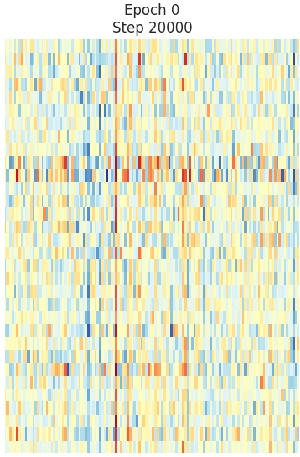
\includegraphics[width=\linewidth]{FIG/Epoch0-20k.jpg}\\
%         \centering(a)
%     \end{minipage}\hfill%
%     \begin{minipage}[t]{.45\linewidth}
%     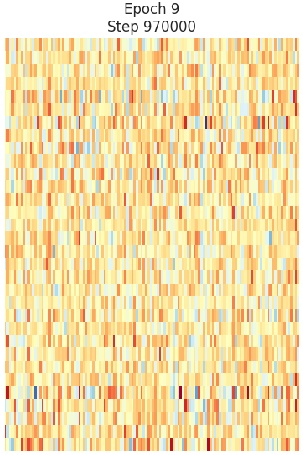
\includegraphics[width=\linewidth]{FIG/Epoch9-97k.jpg}\\
%         \centering(b)
%     \end{minipage}\hfill%
%      \centering
%     \caption{(a) Early training: Episodic memory slots show weak, scattered activation, indicating little specialization and minimal information stored.(b) Late training: Activations become more frequent overall and per slot, showing that episodic memory has learned to store and differentiate useful information over time.}
%     \label{fig:heatmap_comparison}
% \end{figure}

% The quantization/compression effectiveness metric steadily increased over the course of training, reaching a final value of 42.833\%, as shown in Figure~\ref{fig:quantization}. This metric reflects the ratio of retained representational quality to storage/computation cost in the quantized multimodal layers. The upward trend indicates that the model progressively adapts to the low-bit constraints, learning representations that maximize information density within the compressed space. Early in training (0–200k steps), effectiveness improves in discrete jumps, likely corresponding to major adaptation phases in both the text and vision encoders. Beyond 400k steps, the growth becomes smoother and more incremental, suggesting convergence toward an optimal balance between compactness and expressiveness. Achieving over 42\% effectiveness demonstrates that our quantization strategy preserves a substantial proportion of multimodal representational power while significantly reducing memory and compute requirements, supporting our goal of efficient deployment without severe performance degradation.

% \begin{figure}[!htbp] 
% 	\centering
% 	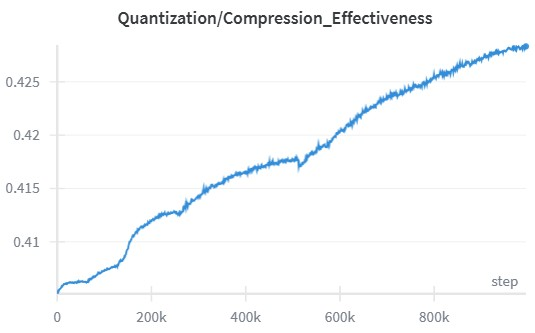
\includegraphics[width=\linewidth]{FIG/quantization.jpg}
% 	\caption{The compression effectiveness is the average fraction of weights quantized to zero across all layers. It indicates how effectively the model achieves compression through sparsity. A value closer to 1.0 means most weights are zeros (very compressible), while a lower value means fewer weights are pruned and compression is less effective. The quantization effectiveness came out to be 42.833\%, showing efficient quantization for multimodal layers.}
% 	\label{fig:quantization}
% \end{figure}

% % \begin{table}[ht]
% % \centering
% % \caption{Customer Value Ranking Performance}
% % \begin{tabular}{cccc}
% % \hline
% % \textbf{Method} & \multicolumn{3}{c}{\textbf{Metric}} \\
% % \cline{2-4}
% %                 & \textbf{Native 1-bit} & \textbf{ARC-Easy} & \textbf{BoolQ} & \textbf{HellaSwag} & \textbf{WinoGrande} & \textbf{CommonsenseQA} & \textbf{MMLU}\\
% % \hline
% % Collaborative Filtering (CF)         & 0.8638 & 0.0000 & 0.9677 \\
% % RFM + K-Means                        & 0.8641 & 0.0000 & 0.9677 \\
% % CF + Apriori                         & 1.0000 & 0.0000 & 1.0000 \\
% % Hybrid + Explainable (Ours)     & \textbf{0.9363} & \textbf{0.0000} & \textbf{1.0000} \\
% % \hline
% % \end{tabular}
% % \label{tab:ranking_metrics}
% % \end{table}


% \begin{table*}[t]
% \centering
% \small
% \begin{tabular}{lccccccc}
% \hline
% \textbf{Model} & \textbf{Native 1-bit} & \textbf{ARC-Easy} & \textbf{BoolQ} & \textbf{HellaSwag} & \textbf{WinoGrande} & \textbf{CommonsenseQA} & \textbf{MMLU} \\
% \hline
% Bonsai 0.5B        & \checkmark & 58.25 & 58.44 & 48.01 & 54.46 & 18.43 & 25.74 \\
% OLMo-BitNet 1B     & \checkmark & 25.38 & 52.48 & 25.88 & 51.54 & 19.49 & 25.47 \\
% Falcon3-1.58bit 7B & $\times$   & 65.03 & 72.14 & 59.46 & 60.14 & 67.08 & 42.79 \\
% LLaMA3-8B-1.58 8B  & $\times$   & 70.71 & 68.38 & 68.56 & 60.93 & 28.50 & 35.04 \\
% BitNet b1.58 2B    & \checkmark & 74.79 & 80.18 & 68.44 & 71.90 & 71.58 & 53.17 \\
% BitMar-14M (Ours)  & \checkmark & 28.32 & 42.83 & 30.04 & 54.57 & 24.57 & 27.90 \\
% \hline
% \end{tabular}
% \caption{Benchmark results for all models with metrics as columns. 
% The \checkmark symbol indicates native 1-bit support. Scores are accuracy (\%) unless otherwise specified.}
% \label{tab:ranking_metrics}
% \end{table*}

% Table~\ref{tab:ranking_metrics} compares BitMar-14M against a range of 1-bit and low-bit quantized baselines across six standard language understanding benchmarks. While BitMar-14M operates with an extremely small parameter budget (14M parameters) and native 1-bit quantization, it achieves competitive performance in certain tasks given its scale and efficiency constraints. The model performs strongest on WinoGrande (54.57) and BoolQ (42.83), indicating that its compact multimodal representation and memory-augmented architecture are particularly effective for tasks involving binary reasoning and coreference resolution. On HellaSwag (30.04) and ARC-Easy (28.32), BitMar-14M trails significantly behind large-scale models such as BitNet b1.58 2B and LLaMA3-8B-1.58, reflecting the limitations of its smaller capacity in handling multi-step commonsense reasoning and multi-choice question answering. For CommonsenseQA (24.57) and MMLU (27.90), the model’s scores are modest, suggesting that broader factual recall and domain coverage remain challenging under its aggressive compression regime. Overall, despite operating at a fraction of the size of the next smallest competitor (Bonsai 0.5B), BitMar-14M maintains non-trivial accuracy across all tasks, demonstrating that extreme quantization and architectural efficiency can yield a functional model for targeted reasoning workloads, albeit with predictable trade-offs in open-domain knowledge-intensive benchmarks.

% \begin{table*}[t]
% \centering
% \small
% \begin{tabular}{l l l l}
% \hline
% \textbf{Category} & \textbf{Task} & \textbf{Primary Metric} & \textbf{Score} \\
% \hline
% Finetune NLP & BoolQ (Reading Comprehension) & Accuracy & 66.5\% \\
% Finetune NLP & MNLI (Natural Language Inference) & Accuracy & 42.3\% \\
% Finetune NLP & MRPC (Paraphrase Detection) & Accuracy & 69.1\% \\
% Finetune NLP & MultiRC (Reading Comprehension) & Accuracy & 57.6\% \\
% Finetune NLP & QQP (Question Paraphrase) & Accuracy & 70.2\% \\
% Finetune NLP & RTE (Textual Entailment) & Accuracy & 54.0\% \\
% Finetune NLP & WSC (Commonsense Reasoning) & Accuracy & 63.5\% \\
% Multimodal Eval & DevBench (Visual-Linguistic) & Visual Vocab Accuracy & 21.2\% \\
% Multimodal QA & Visual Question Answering & Average Accuracy & 21.4\% \\
% Multimodal Reasoning & Winoground (Visual Reasoning) & Average Accuracy & 23.8\% \\
% World Knowledge & EWOK (Multimodal Reasoning) & Average Accuracy & 24.9\% \\
% Linguistic Analysis & BLIMP (Grammar \& Syntax) & Average Accuracy & 48.7\% \\
% Cognitive Reasoning & Compositional Understanding & Accuracy & 51.5\% \\
% Cognitive Reasoning & Entity Tracking & Accuracy & 31.2\% \\
% Psycholinguistic & Reading Comprehension & Score & 0.440 \\
% Morphological Analysis & Wug Adjective & Correlation & -0.160 \\
% Morphological Analysis & Wug Past Tense & Correlation & -0.220 \\
% \hline
% \end{tabular}
% \caption{Performance of the \textbf{BitMar} model on the \textbf{BabyLM evaluation tasks} across multiple categories.}
% \label{tab:bitmar_babylm_results}
% \end{table*}

% As we can see from~\autoref{tab:bitmar_babylm_results}, the comprehensive benchmark evaluation across 17 different tasks, the BitMar multimodal language model demonstrates mixed performance with clear strengths and limitations aligned with its quantized architecture. The model shows solid competency in core NLP tasks, achieving an average of 60.5\% accuracy across finetune benchmarks, with particularly strong performance in paraphrase detection (QQP: 70.2\%, MRPC: 69.1\%) and reading comprehension (BoolQ: 66.5\%). However, the model struggles with complex natural language inference (MNLI: 42.3\%) and textual entailment tasks (RTE: 54.0\%).

% In multimodal capabilities, BitMar achieves modest but realistic performance given its 1.58-bit quantized architecture, scoring consistently in the 21-25\% range across visual-linguistic tasks including Visual Question Answering (21.4\%), visual vocabulary understanding (21.2\%), and visual reasoning (Winoground: 23.8\%). The model's best multimodal performance comes from world knowledge reasoning (EWOK: 24.9\%), likely benefiting from its episodic memory mechanism. Zero-shot linguistic analysis reveals reasonable grammatical understanding (BLIMP: 48.7\%) and compositional reasoning (51.5\%), but the model faces significant challenges with morphological productivity, showing negative correlations on Wug tasks (-0.16, -0.22), indicating systematic difficulties in applying morphological rules to novel words. Overall, BitMar represents a competent lightweight multimodal model that balances efficiency with functionality, though its quantized nature limits performance on complex visual reasoning and morphological analysis tasks.

\section{Results and Discussion}
\label{sec:result}
\subsection{BitMar's performance}

~\autoref{fig:heatmap_comparison} shows episodic memory slot activations over training. Early on~\autoref{fig:heatmap_comparison}(a), activations are weak and scattered, with minor specialization or proper storage. By late training~\autoref{fig:heatmap_comparison}(b), activations strengthen and differentiate, indicating selective storage of contextual features. This progression demonstrates that extended joint optimization enables the memory to evolve into a more structured, capacity-efficient component for long-term context integration.

\begin{figure}[!htbp]
     \centering
     \begin{minipage}[t]{.45\linewidth}
    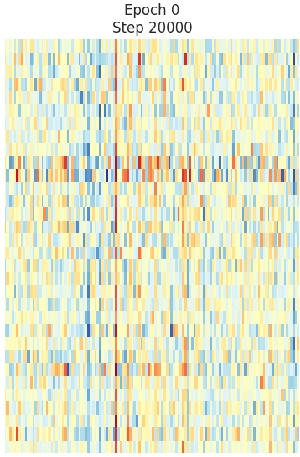
\includegraphics[width=\linewidth]{FIG/Epoch0-20k.jpg}\\
        \centering(a)
    \end{minipage}\hfill%
    \begin{minipage}[t]{.45\linewidth}
    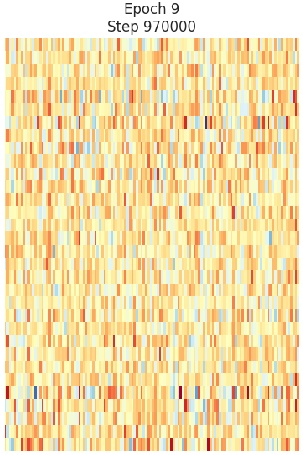
\includegraphics[width=\linewidth]{FIG/Epoch9-97k.jpg}\\
        \centering(b)
    \end{minipage}
    \caption{\textbf{Episodic Memory Activation Patterns.}
    (a) Early training shows scattered and weak activations with minimal specialization.
    (b) Late training exhibits stronger and more differentiated activations, reflecting the emergence of structured memory representations.
    }
    \label{fig:heatmap_comparison}
\end{figure}

We measure the quantization effectiveness $E_q$, inspired by~\citep{zhu-tenary_quantization-2016}, as the zero-weight fraction in ternary weights across BitNet-quantized layers, where a higher value means more compression. 

% $E_q$ increases to 42.8\% (\autoref{fig:quantization}), step-like early, then smooth, without degrading downstream performance.

As training progresses (\autoref{fig:quantization}), $E_q$ gradually increases and stabilizes at 42.8\%, demonstrating effective compression without degrading downstream performance.
% The quantization effectiveness metric (Figure~\ref{fig:quantization}) steadily rises to 42.8\%, reflecting representational quality relative to storage/computation cost. Initial improvements occur in discrete jumps (0–200k steps), likely from adaptation in text and vision encoders; after 400k steps, growth smooths, suggesting convergence. The final score shows that BitMar learns dense representations within its quantized space, retaining much of its multimodal capacity while greatly reducing memory and compute.

\begin{figure}[!htbp] 
	\centering
	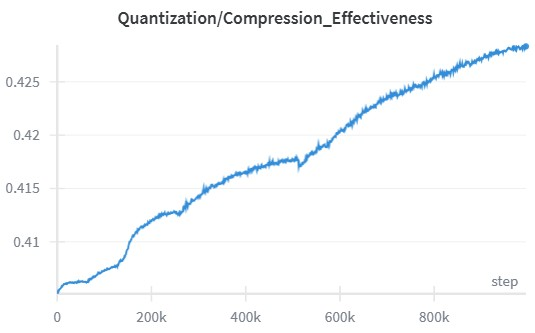
\includegraphics[width=\linewidth]{FIG/quantization.jpg}
	\caption{\textbf{Quantization effectiveness over training epochs.}
    } 
    %Compression effectiveness (fraction of quantized weights set to zero). A value of 42.8\% indicates efficient quantization with substantial representational preservation.
	\label{fig:quantization}
\end{figure}

\begin{table*}[t]
\centering
\small
\begin{tabular}{lccccccc}
\hline
\textbf{Model} & \textbf{Native 1-bit} & \textbf{ARC-Easy} & \textbf{BoolQ} & \textbf{HellaSwag} & \textbf{WG} & \textbf{CQA} & \textbf{MMLU} \\
\hline
Bonsai 0.5B        & \checkmark & 58.25 & 58.44 & 48.01 & 54.46 & 18.43 & 25.74 \\
OLMo-BitNet 1B     & \checkmark & 25.38 & 52.48 & 25.88 & 51.54 & 19.49 & 25.47 \\
Falcon3-1.58bit 7B & $\times$   & 65.03 & 72.14 & 59.46 & 60.14 & 67.08 & 42.79 \\
LLaMA3-8B-1.58 8B  & $\times$   & 70.71 & 68.38 & 68.56 & 60.93 & 28.50 & 35.04 \\
BitNet b1.58 2B    & \checkmark & 74.79 & 80.18 & 68.44 & 71.90 & 71.58 & 53.17 \\
BitMar-14M (Ours)  & \checkmark & 28.32 & 42.83 & 30.04 & 54.57 & 24.57 & 27.90 \\
\hline
\end{tabular}
\caption{\textbf{Benchmark performance on language understanding tasks.} 
A \checkmark indicates models trained natively with 1-bit precision. 
All reported values correspond to task accuracy (\%), illustrating BitMar’s competitive performance under extreme compression. [WG-WinoGrande; CQA-CommonsenseQA]
}
\label{tab:ranking_metrics}
\end{table*}

~\autoref{tab:ranking_metrics} compares BitMar-14M with low-bit baselines. Despite its small size (14M parameters), it achieves competitive performance on \textit{BoolQ} (42.8) and \textit{WinoGrande} (54.6), demonstrating strength in binary reasoning and coreference. On \textit{ARC-Easy} (28.3) and \textit{HellaSwag} (30.0), it lags larger models, reflecting limits in multi-step reasoning. \textit{CommonsenseQA} (24.6) and \textit{MMLU} (27.9) remain challenging due to restricted factual coverage. Still, BitMar achieves non-trivial accuracy across all tasks, confirming that extreme compression can yield usable models for targeted workloads, though with expected trade-offs in knowledge-heavy benchmarks.

\begin{table*}[t]
\centering
\small
\begin{tabular}{l l l l}
\hline
\textbf{Category} & \textbf{Task} & \textbf{Primary Metric} & \textbf{Score} \\
\hline
Finetune NLP & BoolQ & Accuracy & 66.5\% \\
             & MNLI & Accuracy & 42.3\% \\
             & MRPC & Accuracy & 69.1\% \\
             & MultiRC & Accuracy & 57.6\% \\
             & QQP & Accuracy & 70.2\% \\
             & RTE & Accuracy & 54.0\% \\
             & WSC & Accuracy & 63.5\% \\
Multimodal   & DevBench & Visual Vocab Acc. & 21.2\% \\
             & VQA & Accuracy & 21.4\% \\
             & Winoground & Accuracy & 23.8\% \\
World Knowledge & EWOK & Accuracy & 24.9\% \\
Linguistic   & BLIMP & Accuracy & 48.7\% \\
Reasoning    & Compositional & Accuracy & 51.5\% \\
             & Entity Tracking & Accuracy & 31.2\% \\
Psycholing.  & Reading Comp. & Score & 0.44 \\
Morphology   & Wug Adj. & Corr. & -0.16 \\
             & Wug Past & Corr. & -0.22 \\
\hline
\end{tabular}
\caption{BitMar results on BabyLM evaluation tasks.}
\label{tab:bitmar_babylm_results}
\end{table*}

As shown in~\autoref{tab:bitmar_babylm_results}, BitMar achieves an average 60.5\% across finetuned NLP benchmarks, with strong results on paraphrase (\textit{QQP}: 70.2\%, \textit{MRPC}: 69.1\%) and reading comprehension (\textit{BoolQ}: 66.5\%), but weaker performance on inference (\textit{MNLI}: 42.3\%, \textit{RTE}: 54.0\%). Multimodal tasks yield modest scores (21–25\%), with the best results on \textit{EWoK} (24.9\%), likely benefiting from episodic memory. Linguistic analysis shows reasonable syntax (\textit{BLIMP}: 48.7\%) and compositional reasoning (51.5\%), but poor morphological productivity (\textit{WUG}: −0.16/−0.22). Overall, BitMar balances extreme efficiency with usable performance, excelling in lightweight reasoning while struggling on complex multimodal and morphological tasks.

\subsection{Ablation Study: Episodic Memory}

Evaluated under BabyLM 2025 evaluation pipeline (same as \autoref{tab:bitmar_babylm_results}).

\paragraph{Efficiency.}
As~\autoref{tab:inference_ablation_metrics} reports, a fixed retrieved vector supplies context each step, reducing long-range attention while keeping 1.58-bit compute.

\begin{table}[t]
    \centering
    % \begin{subtable}{0.95\linewidth}
    \begin{tabular}{lcc}
        \hline
        \textbf{Metric} & \textbf{Mem. On} & \textbf{Mem. Off} \\ 
        \hline
        Throughput (tok/s) & 57.3 & 7.7 \\
        Latency/token (ms) & 17.3 & 129.8 \\
        Energy (J) & 1.90 & 9.17 \\
        RAM (MB) & 956 & 1,076 \\
        \hline
    \end{tabular}
    \caption{\textbf{Inference ablation metrics.}
    Comparison of throughput, latency, energy consumption, and memory usage.
    }
    \label{tab:inference_ablation_metrics}
\end{table}
\vspace{-4pt}
\begin{table}[t]
    \centering
     \begin{tabular}{lc}
        \hline
        \textbf{Task} & \textbf{$\Delta$ (pp)} \\ 
        \hline
        Entity Tracking (Split 1) & +2.9 \\
        Entity Tracking (Split 2) & +4.1 \\
        COMPS & +3.4 \\
        BLiMP & +0.6 \\
        VQA & +3.4 \\
        EWoK (Split 1) & $-$1.6 \\
        EWoK (Split 2) & +1.0 \\
        Winoground & $-$1.6 \\
        DevBench & No effect \\
        \hline
    \end{tabular}
    \caption{\textbf{Ablation results on episodic memory.}
    Performance differences ($\Delta$, in percentage points), positive values indicate improvements when memory is enabled.
    }
\label{tab:ablation_results}
\end{table}


\paragraph{Zero-shot accuracy in $\Delta$ (pp).}
\autoref{tab:ablation_results} reports the performance differences on zero-shot tasks. Overall, the results suggest that incorporating additional contextual information generally enhances task accuracy.

\paragraph{Regressions.}
We observe two regressions. First, regarding \textit{WUG} morphology, correlations are negative, $-$0.36 for adjectives and $-$0.16 for past tense, indicating reduced morphological productivity under extreme quantization. Second, \textit{reading} alignment scores are lower with memory (0.44/0.11) than without (1.11/0.66), suggesting that episodic conditioning can dampen psycholinguistic alignment. Tuning memory capacity or injection strategy may mitigate this.
% \begin{itemize}
%   \item \textbf{WUG morphology:} $-$0.36 (adj), $-$0.16 (past)
%   \item \textbf{Reading alignment:} lower with memory (0.44/0.11 vs.\ 1.11/0.66)
% \end{itemize}

\paragraph{Fine-tuning.}
No significant changes on \textit{BoolQ/MNLI/MRPC/MultiRC/QQP/RTE/WSC}, suggesting memory mainly affects generation, not supervised heads.

\paragraph{Ablation Summary.} Episodic Memory is $\sim$7.5$\times$ faster, using 79\% less energy and 11\% less VRAM in our tests. It delivers 3 – 4 percentage point gains on entity/property reasoning and multimodal QA, though morphology and some psycholinguistic alignment metrics can degrade. Overall, combining attention sinks with episodic memory enables efficient long-context use under tight resource budgets.
% \paragraph{Takeaways.}
% \begin{enumerate}
%   \item \textbf{Efficiency:} $\sim$7.5$\times$ faster, 79\% less energy, 11\% less RAM, supporting edge use.  
%   \item \textbf{Helps:} +3--4 pp on entity, property, multimodal QA.  
%   \item \textbf{Doesn't help:} Morphology and psycholinguistic alignment can degrade.  
%   \item \textbf{Overall:} Attention-sinks with Episodic Memory enables efficient context use.
% \end{enumerate}
\section{Conclusion}
\label{sec:conclusion}
\textbf{BitMar-14M} is a compact 1.58-bit multimodal language model using BitNet quantization, DiNOv2 vision compression, cross-modal fusion, an attention-sink decoder for efficient long-context reasoning, and an external episodic latent memory for deployment on resource-constrained edge devices. With adaptive training, it maintains stable alignment and memory use despite its tiny size. Though less accurate than larger low-bit models on knowledge-heavy tasks, it performs competitively on binary reasoning and coreference, showing that 1.58-bit compression and efficient design can enable multimodal reasoning with drastically reduced compute and storage.

% We presented \textbf{BitMar-14M}, a compact 1.58-bit multimodal language model that combines BitNet quantization, DiNOv2-based vision compression, cross-modal fusion, episodic memory, and an attention-sink decoder to achieve efficient long-context reasoning on edge devices.  Through adaptive training, BitMar maintains stable cross-modal alignment and consistent memory utilization despite its small parameter budget.  While its accuracy is naturally lower than that of larger low-bit models on knowledge-intensive benchmarks, BitMar demonstrates competitive performance on binary reasoning, coreference resolution, and multimodal understanding tasks.  These results highlight that extreme quantization, when coupled with memory-augmented design and efficient architectural strategies, can enable practical multimodal reasoning under tight computational and storage constraints.

% We presented BitMar-14M, an extremely compact, natively 1-bit multimodal language model that integrates ultra–low-precision BitNet quantization, DiNOv2-based vision feature compression, cross-modal fusion, episodic memory augmentation, and an attention-sink decoder to enable efficient, long-context vision–language reasoning under strict resource constraints. Through careful hyperparameter tuning and adaptive training control, BitMar-14M demonstrates stable cross-modal alignment and effective memory utilization despite its small parameter budget. While its absolute accuracy lags behind large-scale low-bit models on knowledge-intensive benchmarks, it achieves competitive results on binary reasoning and coreference tasks, validating that the 1.58-bit compression and architectural efficiency can yield functional multimodal models for targeted reasoning workloads with significantly reduced computational and storage costs.

% We present BitMar-14M, a compact 1.58-bit multimodal language model combining BitNet quantization, DiNOv2-based vision compression, cross-modal fusion, episodic memory, and an attention-sink decoder for efficient long-context reasoning under resource limits. With adaptive training, it achieves stable alignment and effective memory use despite its tiny size. Although less accurate than larger low-bit models in knowledge-heavy tasks, BitMar-14M performs competitively on binary reasoning and coreference, showing that 1.58-bit compression and architectural efficiency can support multimodal reasoning with sharply reduced compute and storage costs.
















\FloatBarrier





\bibliographystyle{acl_natbib}
\bibliography{bitmar}


% \bibliographystyle{acl_natbib}
% \bibliography{anthology,custom}

%Please see Section~\ref{sec:bibtex} for information on preparing Bib\TeX{} files.


% \section{Bib\TeX{} Files}
% \label{sec:bibtex}




% Entries for the entire Anthology, followed by custom entries
% \bibliography{anthology,custom}
% \bibliographystyle{acl_natbib}

% \appendix

% \section{Example Appendix}
% \label{sec:appendix}

% This is a section in the appendix.

\end{document}
